\documentclass[12pt]{article}
\usepackage[utf8]{inputenc}
\usepackage{amsmath,amsfonts,amssymb}
\usepackage{graphicx}
\usepackage{geometry}
\usepackage{tikz}
\usetikzlibrary{arrows.meta, positioning}
\usepackage{pgfplots}
\pgfplotsset{compat=1.18}
\usepackage{listings}
\usepackage{xcolor}
\geometry{a4paper, margin=1in}
\usepackage{booktabs}
\usepackage{natbib}
\usepackage{noto}
\setcitestyle{authoryear,open={(},close={)}}
\lstset{
  basicstyle=\ttfamily\footnotesize,
  frame=single,
  breaklines=true,
  breakatwhitespace=true,
  columns=flexible,
  numbers=left,
  numberstyle=\tiny,
  keywordstyle=\color{blue}
}

\title{Non-Markovian Generative Influence: A Unified Framework for Cognition, Cosmology, and Spectroscopy}
\author{Flyxion}
\date{September 2025}

\begin{document}

\maketitle

\begin{abstract}
This manuscript proposes a unified framework where memory is modeled as a non-Markovian generative influence process, characterized by autoregressive dynamics with continuous, history-dependent kernels. We integrate the Recognition-Augmented Transformer (RAT) framework \citep{Barenholtz2025}, the Rapid Serial Visual Presentation (RSVP) cosmological model \citep{PacucciLoeb2025}, and Payne-Gaposchkin’s thermodynamic spectroscopy \citep{Payne1925} to demonstrate that cognitive states, galactic spin evolution, and spectral line formation are governed by analogous autoregressive mechanisms. By formalizing influence kernels $K(\Delta t)$, we derive cross-domain mappings that connect cognitive cue activations, cosmic entropy damping, and thermodynamic response functions. Contributions include a novel entropic damping closure for little red dots (LRDs), discriminative predictions against $\Lambda$CDM \citep{MoMaoWhite1998}, and applications to cognitive pathology. Predictions encompass halo-spin decoupling, filament entropy alignment, spectral-entropy correlations, and cognitive influence metrics, testable via JWST \citep{Kocevski2025} and neuroimaging \citep{Barenholtz2025}.
\end{abstract}

\section{Introduction}
\subsection{Background}
Memory underpins diverse disciplines, from cognitive science to cosmology and spectroscopy. Traditional models treat memory as static storage: cognitive science employs discrete buffers \citep{AtkinsonShiffrin1968}, cosmology assumes primordial conditions encode structure formation \citep{EisensteinLoeb1995}, and spectroscopy interprets spectral lines as fixed compositions \citep{Payne1925}. These paradigms struggle with continuous, history-dependent phenomena, such as amnesia’s procedural retention \citep{AtkinsonShiffrin1968}, the dynamical quenching of galactic spins \citep{PacucciLoeb2025}, and entropy-driven spectral features \citep{Maiolino2025}. A unified framework, rooted in non-Markovian autoregressive dynamics, is proposed to reconcile these domains, integrating the Recognition-Augmented Transformer (RAT) \citep{Barenholtz2025}, RSVP cosmology \citep{PacucciLoeb2025}, and thermodynamic spectroscopy \citep{Payne1925}.

\subsection{Description}
We model memory as a generative influence process, where past states exert weighted, non-Markovian effects on future states via autoregressive kernels. This framework unifies cognitive RAT, where cue activations drive state transitions \citep{Barenholtz2025}, RSVP cosmology, where entropy gradients dampen spins \citep{PacucciLoeb2025}, and spectroscopy, where thermodynamic equilibria generate line strengths \citep{Payne1925}. By formalizing cross-domain mappings, we provide a rigorous mathematical structure for memory as continuous influence.

\subsection{Mathematical Formalism}
A non-Markovian autoregressive process is defined as:
\begin{equation}
x_{t+1} = f(x_t, x_{t-1}, \dots; \theta) + \epsilon_t,
\end{equation}
with influence kernel:
\begin{equation}
K(\Delta t) = \frac{\partial x_t}{\partial x_{t-\Delta t}}.
\end{equation}
The memory depth is:
\begin{equation}
D_{\rm mem} = \sum_{\Delta t=1}^\infty K(\Delta t).
\end{equation}
This formalism applies across domains, with $x_t$ representing cognitive states, spin parameters, or ionization numbers \citep{Barenholtz2025, PacucciLoeb2025, Payne1925}.

\section{Modal Memory Models}
\subsection{Background}
Modal memory models, rooted in the cognitive revolution, describe memory as discrete storage systems. Ebbinghaus’s forgetting curves (1885) quantified exponential decay \citep{Ebbinghaus1885}, Bartlett’s reconstructive memory (1932) emphasized schemas \citep{Bartlett1932}, Craik and Lockhart’s levels of processing (1972) prioritized encoding depth \citep{CraikLockhart1972}, and Baddeley’s working memory model (1974) introduced phonological and visuospatial components \citep{Baddeley1974}. The Atkinson-Shiffrin model (1968) formalized sensory, short-term (STM), and long-term memory (LTM) stores \citep{AtkinsonShiffrin1968}, influencing research on amnesia and serial position effects.

\subsection{Description}
Modal models posit a linear flow: sensory inputs enter STM (capacity $\sim 7 \pm 2$ items), consolidate to LTM via rehearsal, and are retrieved via queries \citep{AtkinsonShiffrin1968}. This archival structure assumes discrete boundaries, akin to computational memory.

\subsection{Mathematical Formalism}
STM is modeled as:
\begin{equation}
M_{\rm STM}(t) = \sum_{i=1}^{k} w_i I_i e^{-\alpha (t - t_i)},
\end{equation}
with interference:
\begin{equation}
M_{\rm int}(t) = M_{\rm STM}(t) - \beta \sum_{j \neq i} I_j,
\end{equation}
and processing depth:
\begin{equation}
M_{\rm LTM} \propto \int d(t) dt.
\end{equation}
These models fail to capture continuous influence \citep{Barenholtz2025}.

\begin{table}
\centering
\caption{Comparison of Memory Models}
\begin{tabular}{lcc}
\toprule
\textbf{Model} & \textbf{Form} & \textbf{Limitation} \\
\midrule
Ebbinghaus & $R(t) = e^{-\alpha t}$ & Ignores interference \\
Bartlett & Schemas & Qualitative \\
Craik-Lockhart & $M \propto \int d(t) dt$ & Static encoding \\
Baddeley & Buffers & Discrete limits \\
Atkinson-Shiffrin & $M_{\rm STM} = \sum w_i I_i e^{-\alpha t}$ & Buffer drop-offs \\
Autoregressive & $x_{t+1} = f(x_t, \theta) + \epsilon_t$ & Validation needed \\
\bottomrule
\end{tabular}
\label{tab:memory_models}
\end{table}

\section{Autoregressive Cognition with RAT}
\label{sec:rat_cognition}
\subsection{Background}
The Recognition-Augmented Transformer (RAT) extends autoregressive cognition by integrating cue-driven relevance fields \citep{Barenholtz2025}. Unlike modal models \citep{AtkinsonShiffrin1968}, RAT treats memory as generative, with past states influencing future ones via continuous kernels.

###{Description}
RAT models cognitive states as:
\begin{equation}
x_{t+1} = f(x_t, \theta) + \epsilon_t,
\end{equation}
with relevance fields:
\begin{equation}
R(x) = \sum_i \alpha_i e^{-\|x - \mu_i\|^2 / 2\sigma^2},
\end{equation}
and cue activations:
\begin{equation}
A_c(x) = \phi(\|x - x_c\|) w_c.
\end{equation}
The gradient flow is:
\begin{equation}
\frac{dx}{dt} = f(\nabla R(x), \theta).
\end{equation}
The influence kernel $K(\Delta t)$ reflects cue decay, with memory depth $D_{\rm mem}$ \citep{Barenholtz2025}.

\subsection{Mathematical Formalism}
The kernel is:
\begin{equation}
K(\Delta t) \sim \exp(-\Delta t / \tau_{\rm mem}),
\end{equation}
with transformer self-attention:
\begin{equation}
\text{Attention}(Q,K,V) = \text{softmax}\left(\frac{QK^T}{\sqrt{d_k}}\right)V.
\end{equation}
This unifies cognitive and LLM dynamics \citep{Barenholtz2025}.

\section{RSVP Cosmology}
\label{sec:rsvp_lrd}
\subsection{Background}
RSVP reinterprets galaxy formation as non-Markovian, contrasting $\Lambda$CDM \citep{MoMaoWhite1998}. Alternatives like tidal torque \citep{EisensteinLoeb1995}, merger-driven compaction \citep{Zhuang2025}, and dissipative collapse \citep{BarkanaLoeb2001} assume static spins, but RSVP emphasizes entropic damping \citep{PacucciLoeb2025}.

###{Description}
The spin parameter evolves as:
\begin{equation}
\frac{d\lambda_{\rm eff}}{dt} = -\gamma(\Phi,S,\nabla S,\omega) \lambda_{\rm eff} + \tau_{\rm ext},
\end{equation}
with damping:
\begin{equation}
\gamma(\mathbf{x},t) = \gamma_0 \left(\frac{\Phi}{\Phi_0}\right)^{\alpha} \left(\frac{|\hat{\mathbf{t}}_{\rm fil}\cdot \nabla S|}{|\nabla S|_0}\right)^{\beta} \exp\!\left[-(\omega/\omega_{\rm crit})^\eta\right] + \gamma_{\rm amb}.
\end{equation}
LRDs arise from entropy-driven compaction \citep{PacucciLoeb2025}.

\subsection{Mathematical Formalism}
Compaction occurs when:
\begin{equation}
\int \left[\gamma - \frac{\tau_{\rm ext}}{\lambda_{\rm eff}}\right] dt \gtrsim \ln\left(\frac{\lambda_0}{\lambda_{\rm LRD}}\right).
\end{equation}
At $z=6$, $t_\gamma \sim 0.2 \, \text{Gyr}$ vs. dynamical time $\sim 1 \, \text{Gyr}$.

\section{Thermodynamic Spectroscopy}
\subsection{Background}
Payne-Gaposchkin’s work showed spectra reflect thermodynamic equilibria \citep{Payne1925}, influencing galactic spectroscopy \citep{Maiolino2025}.

###{Description}
Ionization equilibrium is:
\begin{equation}
\frac{n_{i+1}n_e}{n_i} = \frac{2}{\Lambda^3} \frac{g_{i+1}}{g_i} \exp\!\left(-\frac{\chi_i}{kT}\right),
\end{equation}
with kernel:
\begin{equation}
K(\Delta t) \sim \exp\!\left(-\frac{\Delta t}{\tau_{\rm ion}}\right).
\end{equation}
Balmer lines reflect entropy-driven states \citep{Maiolino2025}.

\subsection{Mathematical Formalism}
For Balmer breaks, $n_e \sim 10^9 \, \text{cm}^{-3}$, $T \sim 10^4 \, \text{K}$ yield V-shaped SEDs \citep{Maiolino2025}.

\section{Cross-Domain Mapping}
\subsection{Background}
RAT, RSVP, and spectroscopy share autoregressive cores \citep{Barenholtz2025, PacucciLoeb2025, Payne1925}.

\subsection{Description}
Table \ref{tab:cross_domain} maps domains:
\begin{table}
\centering
\caption{Cross-Domain Autoregressive Mapping}
\begin{tabular}{lcccc}
\toprule
\textbf{Domain} & \textbf{State} & \textbf{Kernel} & \textbf{Cue} & \textbf{Outcome} \\
\midrule
RAT & Cognitive state & $K(\Delta t)$ & Cue activations & Memory, creativity \\
RSVP & $\lambda_{\rm eff}$ & $\gamma$ & Entropy gradients & LRD compactness \\
Spectroscopy & $n_i$ & $K(\Delta t)$ & Entropy field & Balmer lines \\
\bottomrule
\end{tabular}
\label{tab:cross_domain}
\end{table}

\subsection{Mathematical Formalism}
Unified kernel:
\begin{equation}
x_t = \int K(t,s) x_s ds + \epsilon_t.
\end{equation}

\section{Methodology}
\subsection{Background}
Empirical tests contrast RSVP with $\Lambda$CDM \citep{PacucciLoeb2025, Kocevski2025}.

###{Description}
Tests include JWST lensing, CGM tomography, and spectral stacking \citep{Zhuang2025, Maiolino2025}.

\subsection{Mathematical Formalism}
Vorticity spectrum:
\begin{equation}
P_\omega(k) \propto k^{-\alpha}, \quad \alpha \sim 2 \text{ (RSVP)}.
\end{equation}

\section{Case Studies}
\subsection{Background}
Case studies anchor the framework \citep{Barenholtz2025, PacucciLoeb2025, Payne1925}.

###{Description}
H.M., Clive Wearing, LRDs at $z \sim 7$, and Payne’s atmospheres illustrate generative influence.

\subsection{Mathematical Formalism}
Recall probability:
\begin{equation}
P_{\rm recall} \propto K(\Delta t).
\end{equation}

\section{Implications}
\subsection{Background}
The framework connects to predictive coding \citep{Friston2010}, IIT \citep{Tononi2004}, and Bergson’s duration \citep{Bergson1910}.

\subsection{Description}
Memory as constraint enables applications in AI (RAG) and cosmology (CMB anomalies) \citep{Barenholtz2025, PacucciLoeb2025}.

\subsection{Mathematical Formalism}
Free energy:
\begin{equation}
F = \mathbb{E}[\ln p(x|\theta) - \ln q(x)].
\end{equation}

\section{Conclusion}
This framework unifies cognition, cosmology, and spectroscopy via non-Markovian autoregression, with testable predictions \citep{Kocevski2025, Barenholtz2025}.

\begin{figure}
\centering
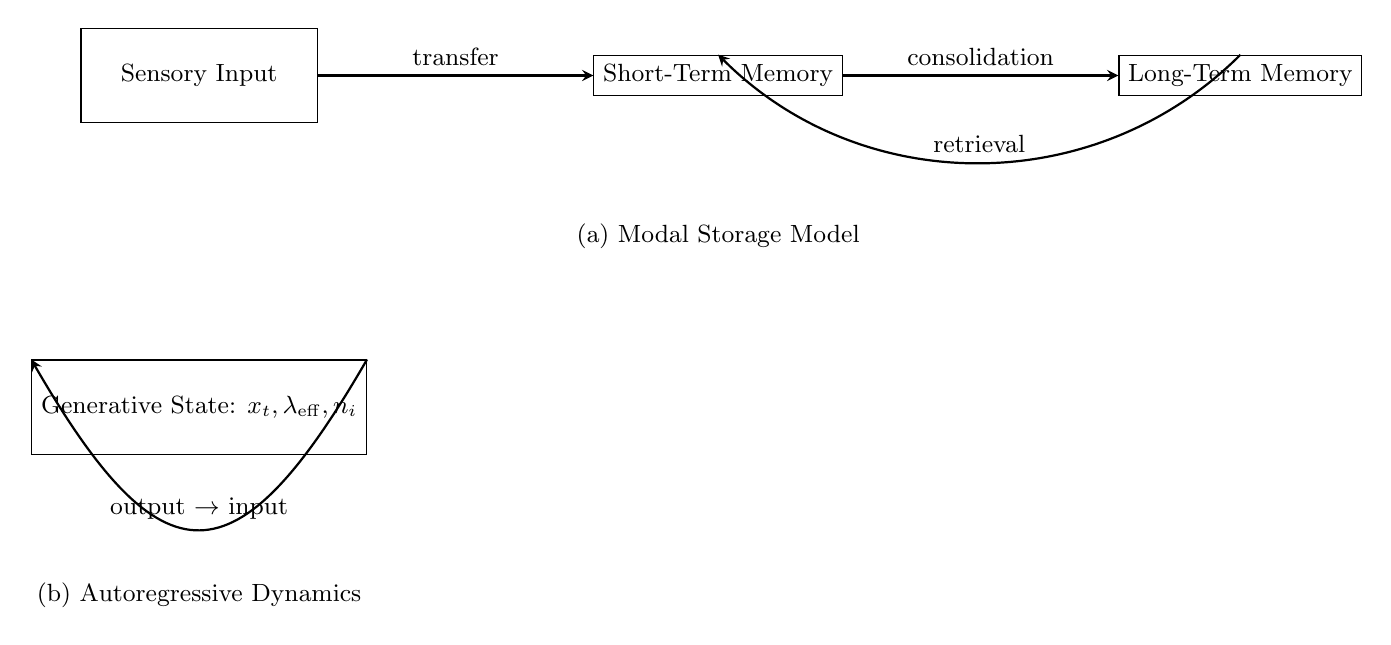
\begin{tikzpicture}[>=stealth, node distance=3cm, every node/.style={font=\small}]
% Panel (a): Modal storage
\node[draw, rectangle, minimum width=3cm, minimum height=1.2cm] (sensory) {Sensory Input};
\node[draw, rectangle, right=3.5cm of sensory] (stm) {Short-Term Memory};
\node[draw, rectangle, right=3.5cm of stm] (ltm) {Long-Term Memory};
\draw[->, thick] (sensory.east) -- (stm.west) node[midway, above] {transfer};
\draw[->, thick] (stm.east) -- (ltm.west) node[midway, above] {consolidation};
\draw[->, thick, bend left=45] (ltm.north) to node[midway, above] {retrieval} (stm.north);
\node[below=1.5cm of stm] {(a) Modal Storage Model};
% Panel (b): Autoregressive
\node[draw, rectangle, minimum width=4cm, minimum height=1.2cm, below=3cm of sensory] (gen) {Generative State: $x_t, \lambda_{\rm eff}, n_i$};
\draw[->, thick, bend left=45] (gen.north east) to [out=60,in=120,looseness=2] node[midway, above] {output $\rightarrow$ input} (gen.north west);
\node[below=1.5cm of gen] {(b) Autoregressive Dynamics};
\end{tikzpicture}
\caption{(a) Modal model \citep{AtkinsonShiffrin1968}. (b) Autoregressive dynamics for RAT, RSVP, and spectroscopy \citep{Barenholtz2025, PacucciLoeb2025, Payne1925}.}
\label{fig:autoregressive}
\end{figure}

\begin{figure}
\centering
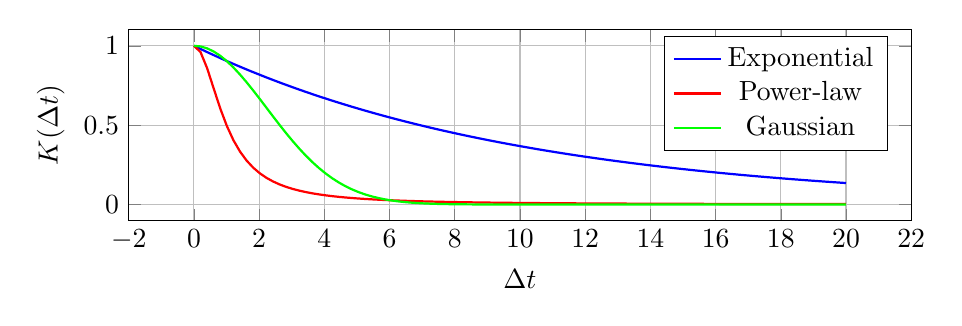
\begin{tikzpicture}
\begin{axis}[
    width=0.95\textwidth,
    height=4cm,
    xlabel={$\Delta t$},
    ylabel={$K(\Delta t)$},
    grid=major,
    domain=0:20,
    samples=100,
    legend pos=north east
]
\addplot[blue, thick] {exp(-x/10)};
\addlegendentry{Exponential}
\addplot[red, thick] {1/(1+x^2)};
\addlegendentry{Power-law}
\addplot[green, thick] {exp(-x^2/10)};
\addlegendentry{Gaussian}
\end{axis}
\end{tikzpicture}
\caption{Influence kernels \citep{Barenholtz2025}.}
\label{fig:kernels}
\end{figure}

\appendix
\section{Stability of RSVP Damping}
\label{app:gamma_closure}
Linearize:
\begin{equation}
\frac{d\delta\lambda}{dt} = -\gamma \delta\lambda.
\end{equation}
Solution: $\delta\lambda(t) = \delta\lambda_0 e^{-\gamma t}$.

\section{Influence Kernels}
\label{app:autoregressive}
Kernels: exponential, power-law, Gaussian. Spectral density:
\begin{equation}
S(f) = \int K(\Delta t) e^{-i2\pi f \Delta t} d\Delta t.
\end{equation}

\section{RAT Formalism}
\label{app:rat}
Relevance fields and cue activations drive $K(\Delta t)$ \citep{Barenholtz2025}.

\section{Cross-Domain Example}
\label{app:example}
For LRDs: $\gamma_0 = 5 \, \text{Gyr}^{-1}$, $\lambda_{\rm LRD} = 0.015$. For RAT: $\tau_{\rm mem} = 10$.

\section{Markov vs. Non-Markov}
\label{app:markov}
Non-Markovian:
\begin{equation}
x(t) = \int_0^t K(t-s) \xi(s) ds.
\end{equation}

\bibliographystyle{plainnat}
\bibliography{references}

\end{document}